\documentclass[a4paper,12pt, leqno]{article}
\usepackage[utf8]{inputenc}
\usepackage[hmargin=2cm,vmargin=2cm]{geometry}
\usepackage[bulgarian]{babel}
\newcommand{\HRule}{\rule{\linewidth}{0.5mm}}
\usepackage{xspace}
\usepackage{amsmath}
\usepackage{verbatim}
\usepackage[unicode]{hyperref}
\hypersetup{
colorlinks=true,
linkcolor=black,
pdftitle={Проект по ASP програминране},
pdfauthor={Валентина Динкова},
pdfsubject={Бази от данни},
pdfcreator={Валентина Динкова}
}
\usepackage{yfonts}
\usepackage{amsthm}
\usepackage {amssymb}
\usepackage{graphicx}
% for source code inclusion
\usepackage{listings}
\renewcommand{\lstlistingname}{\bfseries Файл}


\begin{document}

% TITLE PAGE
\begin{titlepage}
  \begin{center}
СУ „Свети Климент Охридски“ \\
ФМИ
    \\[6cm]
    \HRule \\[0.5cm]

    { \Large \bfseries Проект по ASP програмиране \\ на тема Имоти
    }\\[0.4cm]
    \HRule \\[10cm]


    \begin{minipage}{0.49\textwidth}
      \begin{flushleft} \large
	\emph{Автор:}\\
	Валентина Динкова,\\
	\small ф.н.71112
      \end{flushleft}
    \end{minipage}
    \begin{minipage}{0.49\textwidth}
      \begin{flushright} \large
	\emph{Преподавател:} \\
	доц. д-р Павел Павлов
      \end{flushright}
    \end{minipage}
\\[3cm]
    \vfill
    {\large \today}
  \end{center}
\end{titlepage}

\tableofcontents
\newpage


\section{Задание}
Проектът създава онлайн система за продаване и купуване на имоти. Проектът трябва да обслужва два типа потребители - продавач и купувач. Организацията на работата на системата предполага, че заявката за купуване става дистанционно, а самото купуване се извършва на място.
Продавачът трябва да може да влезе в системата, да добави имот за продаване (с характеристики като квадратура, цена и т.н.), да редактира данните за имот за продаване, да отбелязва имота като продаден. Да може да вижда списък с имоти, които той продава. Да прави справка кои имоти са били продадени.
Купувачът да може да разглежда списък с имоти, да може да прави търсене по квадратура, цена, квартал и др. критерии, да прави заявка за купуване, която да изисква регистрация в системата. Да може да се логва в системата и да вижда списък с имоти, които е заявил за купуване, да добавя имот в списъка, да изтрива имот от списъка. 

  \section{Реализация}
    \subsection{База от данни}

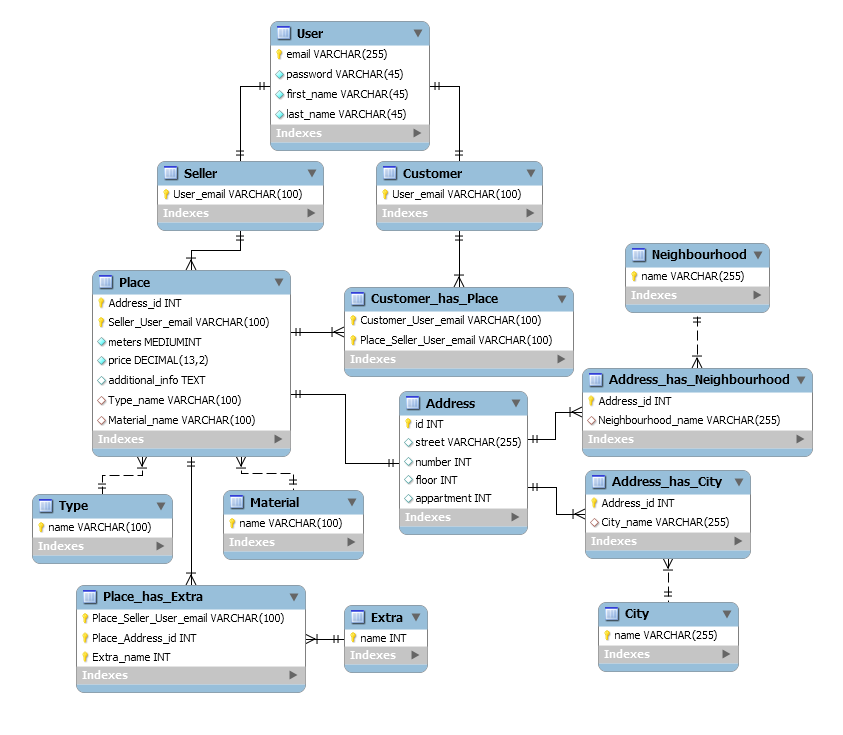
\includegraphics[width=175mm]{diagram.png}
\\
\\
За проекта е използвана система за управление на бази от данни MySQL с ODBC драйвера MyODBC. Кодирането на
символите е UTF-8. На предходната фигура беше представена фигура на релационния модел и следва описание на 
базата от данни.
\\
В базата данни има следните таблици:
\\

\textbf{User} - в нея се пази общата информация за двата вида потребители:
\begin{itemize}
 \item \textit{email} - потребителски e-mail, който е уникален и ще се използва за вход в системата;
 \item \textit{password} - хеширана парола;
 \item \textit{first\_name} - име на потребителя;
 \item \textit{last\_name} - фамилия на потребителя;
 \item \textit{is\_admin} - информация за това дали потребителят е и администратор/продавач (TRUE/FALSE); За да не се прави
заявка, която претърсва цялата таблица Seller, само за да се провери дали даден e-mail е в тази таблица и да се определи
по това дали този потребител е продавач или не.
\end{itemize}

\textbf{Seller и Customer}
\begin{itemize}
 \item \textit{User\_email} - съдържат e-mail на потребителя - външен ключ към User.
\end{itemize}

\textbf{Place}
\begin{itemize}
 \item \textit{Address\_id} - ID на адреса - външен ключ към Address
 \item \textit{Seller\_User\_email} - e-mail на продавача - външен ключ към Seller;
 \item \textit{meters} - квадратура на имота;
 \item \textit{price} - цена на имота;
 \item \textit{additional\_info} - допълнителна информация за имота, която не е задължителна;
 \item \textit{Type\_name} - тип на имота - външен ключ към Type;
 \item \textit{Material\_name} - материал от който е изработен имота - външен ключ към Material;
 \item \textit{Customer\_User\_email} - e-mail на клиента, който е купил имота; ако имота не е купен, стойността на този 
атрибут е NULL.
\end{itemize}

\textbf{Address}
\begin{itemize}
 \item \textit{id} - ID на адреса;
 \item \textit{street} - име на улицата на която се намира имота;
 \item \textit{number} - номер;
 \item \textit{floor} - етаж;
 \item \textit{appartment} - апартамент.
\end{itemize}

\textbf{City}
\begin{itemize}
 \item \textit{name} - име на града;
\end{itemize}

\textbf{Neighbourhood}
\begin{itemize}
 \item \textit{name} - име на квартала;
\end{itemize}

\textbf{Extra}
\begin{itemize}
 \item \textit{name} - допълнителни екстри, като например ТЕЦ;
\end{itemize}

\textbf{Place\_has\_Extra} - таблица, която свързва Place и Extra
\begin{itemize}
 \item \textit{Place\_Address\_id} - външен ключ към Place;
 \item \textit{Extra\_name} - външен ключ към Extra;
\end{itemize}

\textbf{Customer\_has\_Place} - таблица, която свързва Place и Customer; в нея се пази информация 
кои клиенти кои имоти са заявили
\begin{itemize}
 \item \textit{Place\_Address\_id} - външен ключ към Place;
 \item \textit{Extra\_name} - външен ключ към Extra;
\end{itemize}

\textbf{Address\_has\_City} - таблица, която свързва Address и City
\begin{itemize}
 \item \textit{Address\_id} - външен ключ към Address;
 \item \textit{City\_name} - външен ключ към City;
\end{itemize}



\subsection{Приложение}
Скриптовете на приложението са реализирани с \textit{JScript}.
\subsubsection{Помощни файлове}
\begin{itemize}
 \item \textit{md5.inc} - В този файл се намира функция, която хешира паролата на потребителя с md5 алгоритъм.
 \item \textit{helpers.inc} - Помощни функции за форматиране, за работа с масиви, стрингове и т.н.
 \item \textit{connection.inc} - Файл, в който се осъществява връзката с базата данни.
\end{itemize}

\subsubsection{Обща част}
\begin{itemize}
 \item \textit{default.asp} - Началната страница на приложението. Извежда се информация за последно въведените имоти. 
Има възможност за търсене на имот (\textit{search.asp}) по различни критерии. Потребителят може да разглежда и подробно описание 
на имотите (\textit{place.asp}).
 \item \textit{login.asp} - Страница за вписване. Вписването става чрез въвеждане на e-mail и парола.
 \item \textit{logout.asp} - Страница за отписване.
 \item \textit{register.asp} - Страница за регистрация. Потребителят въвежда e-mail, парола, име, фамилия и
какъв вид профил иска - на продавач или на купувач. В зависимост от това какво е избрал (двете са взаимно изключващи се) 
се записва в базата данни в таблицата Seller или Customer.
 \item \textit{place.asp} - Показва подробна информация за даден имот. Ако потребителят е регистриран и 
е влязъл в системата, му се дава възможност да заяви имота за купуване (\textit{add\_place\_list.asp}), а ако не е, 
се изписва, че за да заяви този имот за купуване, е необходимо да има регистрация и да е влязъл в системата.
\end{itemize}


\subsubsection{Част за купувача}
\begin{itemize}
 \item \textit{add\_place\_list.asp} - Позволява добавянето на имот към списъка със заявени за купуване имоти на даден
потребител.
 \item \textit{remove\_place\_list.asp} - Позволява изтриването на имот от списъка със заявени за купуване имоти на 
даден потребител.
 \item \textit{customer\_places\_list.asp} - Позволява на потребителя да разглежда и редактира списък с имотите, 
които е заявил за купуване / вече е купил.
\end{itemize}


\subsubsection{Част за продавача}
\begin{itemize}
 \item \textit{seller\_places\_list.asp} - Позволява на потребителя да разглежда и редактира списък с имоти, които 
продава. Има възможност да види подробната информация, която е въвел, където ще има и възможност да 
види кои са потребителите, заявили този имот за купуване и да избере на кого да бъде продаден имота
 (\textit{choose\_customer.asp}).
 \item \textit{add\_place.asp} - Позволява на потребителя да добавя нови места за продаване.
 \item \textit{remove\_place.asp} - Позволява на потребителя да изтрива места, които е добавил за продаване
 \item \textit{edit\_place.asp} - Позволява на потребителя да редактира информацията за даден имот, 
който е обявил за продаване.
 \item \textit{choose\_customer.asp} - Позволява на потребителя да избере кой потребител да купи имота от списъка със 
заявилите го за купуване и по този начин имота ще се води продаден.
\end{itemize}

За оформяне на дизайна на страниците се използва файл \textit{style.css}.


\end{document}